
The Partition Coloring Problem is a generalization of the Standard Vertex Coloring Problem (VCP) and has initially been considered by Li and Simha in \cite{li-00}. The problem arised from considering the join problem of routing and wavelength assignment in Wavelength Division Multiplexing optical networks. It is therefore a subproblem of a variant of the Wavelength Routing and Assignment Problem (RWA), namly the min-RWA problem. This chapter aims to give formal definitions and examples of VCP, PCP and min-RWA and reason about their computational complexities.

\section{Standard Vertex Coloring Problem}
As the PCP is a generalization of VCP, this section provides a formal defintion.\\
Given a non-directed graph $G=(V,E)$, the VCP consists in assigning a color to each node in $V$, such that no adjancent nodes have the same color. The aim is to minimize the chromatic number, i.e. the overall number of colors used. Figure \ref{pd:vcp} shows the Petersen graph \cite{holton-08}, colored within 3 colors\footnote{Graphic taken from http://en.wikipedia.org/wiki/File:Petersen_graph_3-coloring.svg}.

\begin{figure}
\begin{center}
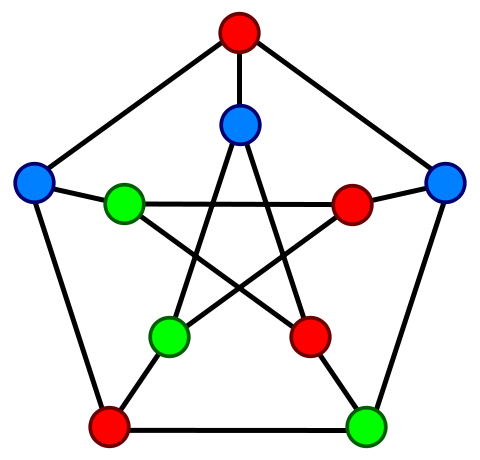
\includegraphics[scale=1]{figures/vcp.png}
\caption{Instance of an optical network with 57 vertices and 85 edges. Extracted from the European optical transport network. \cite{belgacem-13}}
\label{pd:vcp}
\end{center}
\end{figure}

\section{Partition Coloring Problem}

As many Network Design Problems (NDPs), the VCP can be generalized by partitioning the vertex set $V$ into clusters $V_k, k \in K$, and expressing feasability constraints in terms of the clusters instead of individual nodes. \cite{feremans-03} One resulting Generalized Network Design Problem (GNDP) is the PCP, which is due to Fereman's definition an ``Exactly'' GNDP, since it requires the solution to select exactly one vertex per each cluster. In contrast, ``At Least'' and ``At Most'' generalizations aim to select at least, respectively at most a given number of vertices per each cluster. A formal definiton of PCP follows: \\\\
Let $G = (V, E)$ be a non-directed graph and $V$ partitioned into $q$ mutually exclusive, nonempty subsets $V_1, V_2,\ldots, V_q$, where $V_i \cap V_j = \emptyset, \forall i, j = 1, \ldots , q$, $i \neq j$. We refer to $V_1, V_2, \ldots , V_q$ as the components of the partition. The PCP consists in finding a subset $V' \subset V$ such that $|V' \cap V_i| = 1, \forall i = 1, \ldots , q$ (i.e., $V'$ contains one node of each component $V_i$), and the chromatic number of the graph induced in $G$ by $V'$ is minimum.\\\\
Figure \ref{pd:pcpExample} shows an example of an instance with 5 clusters, each holding 2 nodes and its solution with a chromatic number of 2.

\begin{figure}
\begin{center}
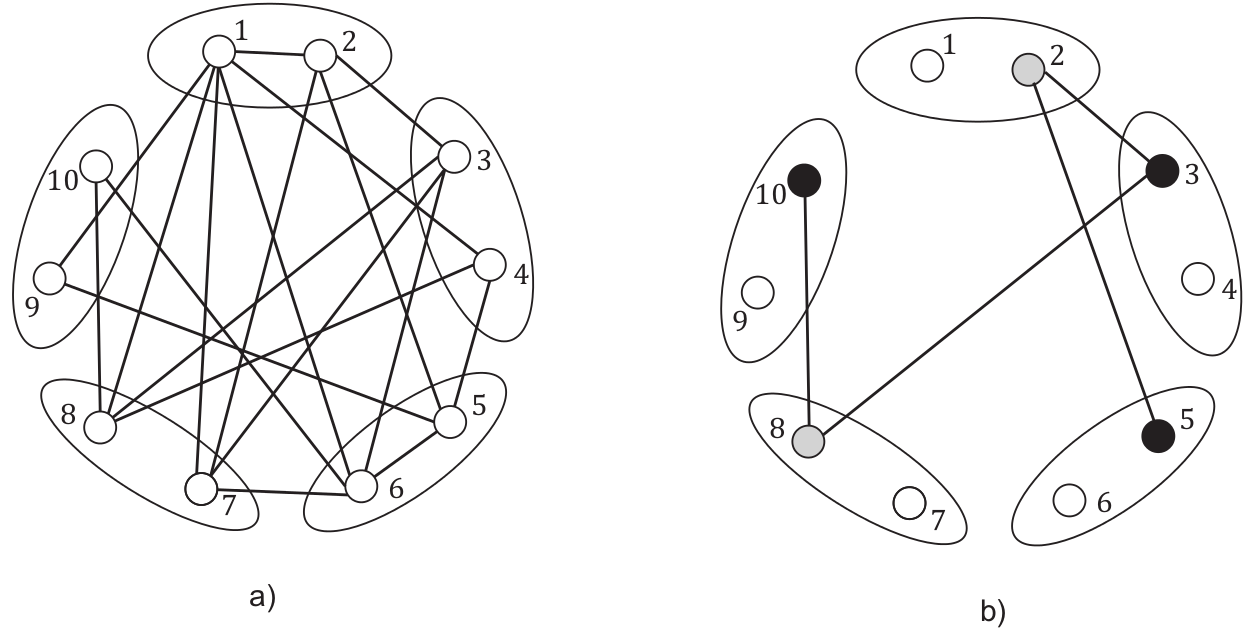
\includegraphics[scale=0.3]{figures/pcp.png}
\caption{a) Shows a problem instance and b) its optimal solution with two colors.}
\label{pd:pcpExample}
\end{center}
\end{figure}


\section{Wavelength Routing and Assignment Problem}

Wavelength Division Multiplexing is a technique that allows a single optical link to transfer multiple datastreams simultaneously by using distinct wavelengths for each datastream. Data is transferred along a route of linked physical network routing devices (nodes). An all optical connection between two nodes is called lightpath. Assuming the so called wavelength continuity constraint \cite{markovic-10} means to assume that the same wavelength has to be kept over all physical links along the route (i.e. it can not be converted by any node), so the lightpath has to be set up with one wavelength from the source to the destination node. It follows that any two paths, having at least one link in common, have to use different wavelengths, in order to enable the common link(s) to transfer data simultaneously. Figure \ref{pd:opticalNetwork} shows an extract of the European optical transport network.\\

\begin{figure}
\begin{center}
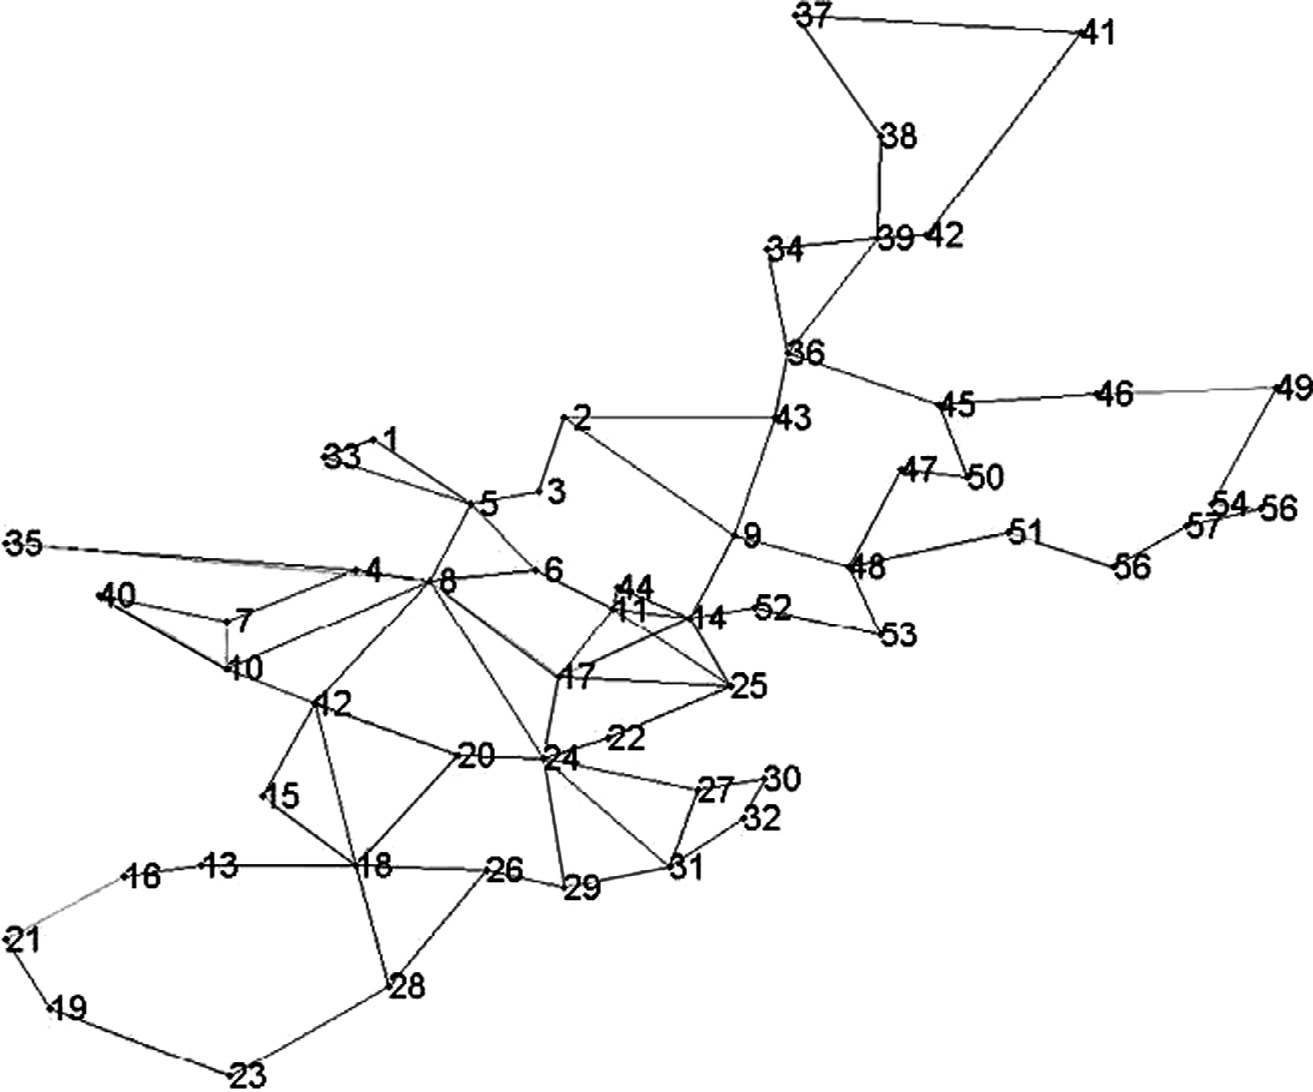
\includegraphics[scale=0.2]{figures/rwa.png}
\caption{Instance of an optical network with 57 vertices and 85 edges. Extracted from the European optical transport network. \cite{belgacem-13}}
\label{pd:opticalNetwork}
\end{center}
\end{figure}
  
In general, the Wavelength Routing and Assignment Problem (RWA) consists of an undirected network Graph $N=(V,E)$, where nodes represent network routing devices and edges represent full duplex (optical) links, i.e. links supporting data transmission in both directions. Further, a set of source-destination pairs (or connection requests) $C=\{(s_1,d_2),\ldots , (s_k, d_k) : s_i,d_i \in V\}$ and a set of wavelengths $\Lambda = \{\alpha_1 , \ldots, \alpha_m \}$ is given. If all connection requests are known in advance, the RWA is said to be static, otherwise dynamic. \cite{murthy-02} The static RWA can further be distinguished by characteristics of its objective. In the context of this thesis, only the min-RWA problem is relevant, which is a static version of RWA aiming to select exactly one path and one wavelength for each pair $(s,d) \in C$, in the way that the number of wavelength $\left\vert{\Lambda}\right\vert$ is minimized under the continuity constraint and its consequences, i.e. if any two paths have at least one edge in common, distinct wavelengths have to be assigned to them. The problem can be split into two subproblems:

\begin{enumerate}
\item routing: finding a set of paths $P_{s,d}$ for each source-destination pair $(s,d) \in C$
\item wavelength assignment: selecting exactly one path in $P_{s,d}$ and one wavelength $\alpha_i$ for each pair $(s,d) \in C$, in the way that the number of wavelength is minimized under the continuity constraint.
\end{enumerate}

Considering the demands of real world instances, it is clear that the computed paths should be relatively short. The first subproblem can be solved in polynomial time by any single source shortest path algorithms like Dijkstra's- or the B*-algorithm. If $\left\vert{P_{s,d}}\right\vert = 1, \forall (s,d)\in C$, i.e. there is exactly one path considered for each source-destination pair, the second subproblem can be transformed into VCP, in any other case $\exists (s,d)\in C : \left\vert{P_{s,d}}\right\vert > 1$ into PCP. The transformation consists in considering each source-destination pair $(s,d)$ as a cluster and and each path in $P_{s,d}$ as a node. In the case that two paths share at least one edge, the corresping nodes are adjacent. Selecting a node-color pair out of a cluster in PCP is equivalent to selecting a path out of a  to a node in PCP is equivalent to Figure \ref{pd:transformation} demonstrates the transformation by example.


\begin{center}
\begin{figure}
\centering
\ifx\du\undefined
  \newlength{\du}
\fi
\setlength{\du}{15\unitlength}
\begin{tikzpicture}
\pgftransformxscale{1.000000}
\pgftransformyscale{-1.000000}
\definecolor{dialinecolor}{rgb}{0.000000, 0.000000, 0.000000}
\pgfsetstrokecolor{dialinecolor}
\definecolor{dialinecolor}{rgb}{1.000000, 1.000000, 1.000000}
\pgfsetfillcolor{dialinecolor}
\pgfsetlinewidth{0.050000\du}
\pgfsetdash{}{0pt}
\pgfsetdash{}{0pt}
\pgfsetbuttcap
\pgfsetmiterjoin
\pgfsetlinewidth{0.050000\du}
\pgfsetbuttcap
\pgfsetmiterjoin
\pgfsetdash{}{0pt}
\definecolor{dialinecolor}{rgb}{1.000000, 1.000000, 1.000000}
\pgfsetfillcolor{dialinecolor}
\pgfpathellipse{\pgfpoint{14.562500\du}{15.212500\du}}{\pgfpoint{0.562500\du}{0\du}}{\pgfpoint{0\du}{0.562500\du}}
\pgfusepath{fill}
\definecolor{dialinecolor}{rgb}{0.000000, 0.000000, 0.000000}
\pgfsetstrokecolor{dialinecolor}
\pgfpathellipse{\pgfpoint{14.562500\du}{15.212500\du}}{\pgfpoint{0.562500\du}{0\du}}{\pgfpoint{0\du}{0.562500\du}}
\pgfusepath{stroke}
\pgfsetbuttcap
\pgfsetmiterjoin
\pgfsetdash{}{0pt}
\definecolor{dialinecolor}{rgb}{0.000000, 0.000000, 0.000000}
\pgfsetstrokecolor{dialinecolor}
\pgfpathellipse{\pgfpoint{14.562500\du}{15.212500\du}}{\pgfpoint{0.562500\du}{0\du}}{\pgfpoint{0\du}{0.562500\du}}
\pgfusepath{stroke}
\pgfsetlinewidth{0.050000\du}
\pgfsetdash{}{0pt}
\pgfsetdash{}{0pt}
\pgfsetbuttcap
\pgfsetmiterjoin
\pgfsetlinewidth{0.050000\du}
\pgfsetbuttcap
\pgfsetmiterjoin
\pgfsetdash{}{0pt}
\definecolor{dialinecolor}{rgb}{1.000000, 1.000000, 1.000000}
\pgfsetfillcolor{dialinecolor}
\pgfpathellipse{\pgfpoint{16.747500\du}{18.662500\du}}{\pgfpoint{0.562500\du}{0\du}}{\pgfpoint{0\du}{0.562500\du}}
\pgfusepath{fill}
\definecolor{dialinecolor}{rgb}{0.000000, 0.000000, 0.000000}
\pgfsetstrokecolor{dialinecolor}
\pgfpathellipse{\pgfpoint{16.747500\du}{18.662500\du}}{\pgfpoint{0.562500\du}{0\du}}{\pgfpoint{0\du}{0.562500\du}}
\pgfusepath{stroke}
\pgfsetbuttcap
\pgfsetmiterjoin
\pgfsetdash{}{0pt}
\definecolor{dialinecolor}{rgb}{0.000000, 0.000000, 0.000000}
\pgfsetstrokecolor{dialinecolor}
\pgfpathellipse{\pgfpoint{16.747500\du}{18.662500\du}}{\pgfpoint{0.562500\du}{0\du}}{\pgfpoint{0\du}{0.562500\du}}
\pgfusepath{stroke}
\pgfsetlinewidth{0.050000\du}
\pgfsetdash{}{0pt}
\pgfsetdash{}{0pt}
\pgfsetbuttcap
\pgfsetmiterjoin
\pgfsetlinewidth{0.050000\du}
\pgfsetbuttcap
\pgfsetmiterjoin
\pgfsetdash{}{0pt}
\definecolor{dialinecolor}{rgb}{1.000000, 1.000000, 1.000000}
\pgfsetfillcolor{dialinecolor}
\pgfpathellipse{\pgfpoint{22.632500\du}{11.112500\du}}{\pgfpoint{0.562500\du}{0\du}}{\pgfpoint{0\du}{0.562500\du}}
\pgfusepath{fill}
\definecolor{dialinecolor}{rgb}{0.000000, 0.000000, 0.000000}
\pgfsetstrokecolor{dialinecolor}
\pgfpathellipse{\pgfpoint{22.632500\du}{11.112500\du}}{\pgfpoint{0.562500\du}{0\du}}{\pgfpoint{0\du}{0.562500\du}}
\pgfusepath{stroke}
\pgfsetbuttcap
\pgfsetmiterjoin
\pgfsetdash{}{0pt}
\definecolor{dialinecolor}{rgb}{0.000000, 0.000000, 0.000000}
\pgfsetstrokecolor{dialinecolor}
\pgfpathellipse{\pgfpoint{22.632500\du}{11.112500\du}}{\pgfpoint{0.562500\du}{0\du}}{\pgfpoint{0\du}{0.562500\du}}
\pgfusepath{stroke}
\pgfsetlinewidth{0.050000\du}
\pgfsetdash{}{0pt}
\pgfsetdash{}{0pt}
\pgfsetbuttcap
\pgfsetmiterjoin
\pgfsetlinewidth{0.050000\du}
\pgfsetbuttcap
\pgfsetmiterjoin
\pgfsetdash{}{0pt}
\definecolor{dialinecolor}{rgb}{1.000000, 1.000000, 1.000000}
\pgfsetfillcolor{dialinecolor}
\pgfpathellipse{\pgfpoint{17.817500\du}{11.912500\du}}{\pgfpoint{0.562500\du}{0\du}}{\pgfpoint{0\du}{0.562500\du}}
\pgfusepath{fill}
\definecolor{dialinecolor}{rgb}{0.000000, 0.000000, 0.000000}
\pgfsetstrokecolor{dialinecolor}
\pgfpathellipse{\pgfpoint{17.817500\du}{11.912500\du}}{\pgfpoint{0.562500\du}{0\du}}{\pgfpoint{0\du}{0.562500\du}}
\pgfusepath{stroke}
\pgfsetbuttcap
\pgfsetmiterjoin
\pgfsetdash{}{0pt}
\definecolor{dialinecolor}{rgb}{0.000000, 0.000000, 0.000000}
\pgfsetstrokecolor{dialinecolor}
\pgfpathellipse{\pgfpoint{17.817500\du}{11.912500\du}}{\pgfpoint{0.562500\du}{0\du}}{\pgfpoint{0\du}{0.562500\du}}
\pgfusepath{stroke}
\pgfsetlinewidth{0.050000\du}
\pgfsetdash{}{0pt}
\pgfsetdash{}{0pt}
\pgfsetbuttcap
\pgfsetmiterjoin
\pgfsetlinewidth{0.050000\du}
\pgfsetbuttcap
\pgfsetmiterjoin
\pgfsetdash{}{0pt}
\definecolor{dialinecolor}{rgb}{1.000000, 1.000000, 1.000000}
\pgfsetfillcolor{dialinecolor}
\pgfpathellipse{\pgfpoint{20.043921\du}{13.577576\du}}{\pgfpoint{0.562500\du}{0\du}}{\pgfpoint{0\du}{0.562500\du}}
\pgfusepath{fill}
\definecolor{dialinecolor}{rgb}{0.000000, 0.000000, 0.000000}
\pgfsetstrokecolor{dialinecolor}
\pgfpathellipse{\pgfpoint{20.043921\du}{13.577576\du}}{\pgfpoint{0.562500\du}{0\du}}{\pgfpoint{0\du}{0.562500\du}}
\pgfusepath{stroke}
\pgfsetbuttcap
\pgfsetmiterjoin
\pgfsetdash{}{0pt}
\definecolor{dialinecolor}{rgb}{0.000000, 0.000000, 0.000000}
\pgfsetstrokecolor{dialinecolor}
\pgfpathellipse{\pgfpoint{20.043921\du}{13.577576\du}}{\pgfpoint{0.562500\du}{0\du}}{\pgfpoint{0\du}{0.562500\du}}
\pgfusepath{stroke}
\pgfsetlinewidth{0.050000\du}
\pgfsetdash{}{0pt}
\pgfsetdash{}{0pt}
\pgfsetbuttcap
\pgfsetmiterjoin
\pgfsetlinewidth{0.050000\du}
\pgfsetbuttcap
\pgfsetmiterjoin
\pgfsetdash{}{0pt}
\definecolor{dialinecolor}{rgb}{1.000000, 1.000000, 1.000000}
\pgfsetfillcolor{dialinecolor}
\pgfpathellipse{\pgfpoint{23.654200\du}{17.479200\du}}{\pgfpoint{0.562500\du}{0\du}}{\pgfpoint{0\du}{0.562500\du}}
\pgfusepath{fill}
\definecolor{dialinecolor}{rgb}{0.000000, 0.000000, 0.000000}
\pgfsetstrokecolor{dialinecolor}
\pgfpathellipse{\pgfpoint{23.654200\du}{17.479200\du}}{\pgfpoint{0.562500\du}{0\du}}{\pgfpoint{0\du}{0.562500\du}}
\pgfusepath{stroke}
\pgfsetbuttcap
\pgfsetmiterjoin
\pgfsetdash{}{0pt}
\definecolor{dialinecolor}{rgb}{0.000000, 0.000000, 0.000000}
\pgfsetstrokecolor{dialinecolor}
\pgfpathellipse{\pgfpoint{23.654200\du}{17.479200\du}}{\pgfpoint{0.562500\du}{0\du}}{\pgfpoint{0\du}{0.562500\du}}
\pgfusepath{stroke}
% setfont left to latex
\definecolor{dialinecolor}{rgb}{0.000000, 0.000000, 0.000000}
\pgfsetstrokecolor{dialinecolor}
\node[anchor=west] at (17.492500\du,11.912500\du){1};
% setfont left to latex
\definecolor{dialinecolor}{rgb}{0.000000, 0.000000, 0.000000}
\pgfsetstrokecolor{dialinecolor}
\node[anchor=west] at (22.332500\du,11.112500\du){2};
% setfont left to latex
\definecolor{dialinecolor}{rgb}{0.000000, 0.000000, 0.000000}
\pgfsetstrokecolor{dialinecolor}
\node[anchor=west] at (17.300000\du,10.250000\du){};
% setfont left to latex
\definecolor{dialinecolor}{rgb}{0.000000, 0.000000, 0.000000}
\pgfsetstrokecolor{dialinecolor}
\node[anchor=west] at (14.262500\du,15.212500\du){3};
% setfont left to latex
\definecolor{dialinecolor}{rgb}{0.000000, 0.000000, 0.000000}
\pgfsetstrokecolor{dialinecolor}
\node[anchor=west] at (19.481421\du,13.577576\du){4};
% setfont left to latex
\definecolor{dialinecolor}{rgb}{0.000000, 0.000000, 0.000000}
\pgfsetstrokecolor{dialinecolor}
\node[anchor=west] at (16.347500\du,18.662500\du){5};
\pgfsetlinewidth{0.050000\du}
\pgfsetdash{}{0pt}
\pgfsetdash{}{0pt}
\pgfsetbuttcap
{
\definecolor{dialinecolor}{rgb}{0.000000, 0.000000, 0.000000}
\pgfsetfillcolor{dialinecolor}
% was here!!!
\definecolor{dialinecolor}{rgb}{0.000000, 0.000000, 0.000000}
\pgfsetstrokecolor{dialinecolor}
\draw (17.407446\du,12.328223\du)--(14.972554\du,14.796777\du);
}
\pgfsetlinewidth{0.050000\du}
\pgfsetdash{}{0pt}
\pgfsetdash{}{0pt}
\pgfsetbuttcap
{
\definecolor{dialinecolor}{rgb}{0.000000, 0.000000, 0.000000}
\pgfsetfillcolor{dialinecolor}
% was here!!!
\definecolor{dialinecolor}{rgb}{0.000000, 0.000000, 0.000000}
\pgfsetstrokecolor{dialinecolor}
\draw (14.931300\du,15.725000\du)--(16.438666\du,18.162996\du);
}
\pgfsetlinewidth{0.050000\du}
\pgfsetdash{}{0pt}
\pgfsetdash{}{0pt}
\pgfsetbuttcap
{
\definecolor{dialinecolor}{rgb}{0.000000, 0.000000, 0.000000}
\pgfsetfillcolor{dialinecolor}
% was here!!!
\definecolor{dialinecolor}{rgb}{0.000000, 0.000000, 0.000000}
\pgfsetstrokecolor{dialinecolor}
\draw (18.287679\du,12.264133\du)--(19.573742\du,13.225942\du);
}
\pgfsetlinewidth{0.050000\du}
\pgfsetdash{}{0pt}
\pgfsetdash{}{0pt}
\pgfsetbuttcap
{
\definecolor{dialinecolor}{rgb}{0.000000, 0.000000, 0.000000}
\pgfsetfillcolor{dialinecolor}
% was here!!!
\definecolor{dialinecolor}{rgb}{0.000000, 0.000000, 0.000000}
\pgfsetstrokecolor{dialinecolor}
\draw (19.508435\du,16.764690\du)--(17.230624\du,18.330411\du);
}
\pgfsetlinewidth{0.050000\du}
\pgfsetdash{}{0pt}
\pgfsetdash{}{0pt}
\pgfsetbuttcap
{
\definecolor{dialinecolor}{rgb}{0.000000, 0.000000, 0.000000}
\pgfsetfillcolor{dialinecolor}
% was here!!!
\definecolor{dialinecolor}{rgb}{0.000000, 0.000000, 0.000000}
\pgfsetstrokecolor{dialinecolor}
\draw (22.207179\du,11.517528\du)--(20.469242\du,13.172547\du);
}
\pgfsetlinewidth{0.050000\du}
\pgfsetdash{}{0pt}
\pgfsetdash{}{0pt}
\pgfsetbuttcap
{
\definecolor{dialinecolor}{rgb}{0.000000, 0.000000, 0.000000}
\pgfsetfillcolor{dialinecolor}
% was here!!!
\definecolor{dialinecolor}{rgb}{0.000000, 0.000000, 0.000000}
\pgfsetstrokecolor{dialinecolor}
\draw (20.553117\du,16.593066\du)--(23.092643\du,17.318735\du);
}
\pgfsetlinewidth{0.050000\du}
\pgfsetdash{}{0pt}
\pgfsetdash{}{0pt}
\pgfsetbuttcap
{
\definecolor{dialinecolor}{rgb}{0.000000, 0.000000, 0.000000}
\pgfsetfillcolor{dialinecolor}
% was here!!!
\definecolor{dialinecolor}{rgb}{0.000000, 0.000000, 0.000000}
\pgfsetstrokecolor{dialinecolor}
\draw (22.831300\du,11.725000\du)--(23.571227\du,16.899004\du);
}
% setfont left to latex
\definecolor{dialinecolor}{rgb}{1.000000, 0.000000, 0.000000}
\pgfsetstrokecolor{dialinecolor}
\node[anchor=west] at (17.297900\du,10.775000\du){s1};
% setfont left to latex
\definecolor{dialinecolor}{rgb}{0.000000, 0.000000, 1.000000}
\pgfsetstrokecolor{dialinecolor}
\node[anchor=west] at (22.510400\du,10.075000\du){s2};
% setfont left to latex
\definecolor{dialinecolor}{rgb}{0.000000, 0.000000, 1.000000}
\pgfsetstrokecolor{dialinecolor}
\node[anchor=west] at (23.310400\du,18.775000\du){d2};
% setfont left to latex
\definecolor{dialinecolor}{rgb}{1.000000, 0.000000, 0.000000}
\pgfsetstrokecolor{dialinecolor}
\node[anchor=west] at (16.610400\du,19.908300\du){d1};
\pgfsetlinewidth{0.050000\du}
\pgfsetdash{{\pgflinewidth}{0.200000\du}}{0cm}
\pgfsetdash{{\pgflinewidth}{0.200000\du}}{0cm}
\pgfsetbuttcap
{
\definecolor{dialinecolor}{rgb}{1.000000, 0.000000, 0.000000}
\pgfsetfillcolor{dialinecolor}
% was here!!!
\definecolor{dialinecolor}{rgb}{1.000000, 0.000000, 0.000000}
\pgfsetstrokecolor{dialinecolor}
\draw (17.611544\du,12.934315\du)--(15.307430\du,15.292183\du);
}
\pgfsetlinewidth{0.050000\du}
\pgfsetdash{{\pgflinewidth}{0.200000\du}}{0cm}
\pgfsetdash{{\pgflinewidth}{0.200000\du}}{0cm}
\pgfsetbuttcap
{
\definecolor{dialinecolor}{rgb}{1.000000, 0.000000, 0.000000}
\pgfsetfillcolor{dialinecolor}
% was here!!!
\pgfsetarrowsend{to}
\definecolor{dialinecolor}{rgb}{1.000000, 0.000000, 0.000000}
\pgfsetstrokecolor{dialinecolor}
\draw (15.278092\du,15.338478\du)--(16.727660\du,17.530509\du);
}
\pgfsetlinewidth{0.050000\du}
\pgfsetdash{{\pgflinewidth}{0.200000\du}}{0cm}
\pgfsetdash{{\pgflinewidth}{0.200000\du}}{0cm}
\pgfsetbuttcap
{
\definecolor{dialinecolor}{rgb}{1.000000, 0.000000, 0.000000}
\pgfsetfillcolor{dialinecolor}
% was here!!!
\definecolor{dialinecolor}{rgb}{1.000000, 0.000000, 0.000000}
\pgfsetstrokecolor{dialinecolor}
\draw (17.925100\du,12.946573\du)--(19.267179\du,14.016979\du);
}
\pgfsetlinewidth{0.050000\du}
\pgfsetdash{{\pgflinewidth}{0.200000\du}}{0cm}
\pgfsetdash{{\pgflinewidth}{0.200000\du}}{0cm}
\pgfsetbuttcap
{
\definecolor{dialinecolor}{rgb}{1.000000, 0.000000, 0.000000}
\pgfsetfillcolor{dialinecolor}
% was here!!!
\pgfsetarrowsend{to}
\definecolor{dialinecolor}{rgb}{1.000000, 0.000000, 0.000000}
\pgfsetstrokecolor{dialinecolor}
\draw (19.379311\du,15.739035\du)--(16.975148\du,17.718934\du);
}
\pgfsetlinewidth{0.050000\du}
\pgfsetdash{{\pgflinewidth}{0.200000\du}}{0cm}
\pgfsetdash{{\pgflinewidth}{0.200000\du}}{0cm}
\pgfsetbuttcap
{
\definecolor{dialinecolor}{rgb}{0.000000, 0.000000, 1.000000}
\pgfsetfillcolor{dialinecolor}
% was here!!!
\definecolor{dialinecolor}{rgb}{0.000000, 0.000000, 1.000000}
\pgfsetstrokecolor{dialinecolor}
\draw (22.480196\du,12.254873\du)--(20.750100\du,13.971573\du);
}
\pgfsetlinewidth{0.050000\du}
\pgfsetdash{{\pgflinewidth}{0.200000\du}}{0cm}
\pgfsetdash{{\pgflinewidth}{0.200000\du}}{0cm}
\pgfsetbuttcap
{
\definecolor{dialinecolor}{rgb}{0.000000, 0.000000, 1.000000}
\pgfsetfillcolor{dialinecolor}
% was here!!!
\pgfsetarrowsend{to}
\definecolor{dialinecolor}{rgb}{0.000000, 0.000000, 1.000000}
\pgfsetstrokecolor{dialinecolor}
\draw (20.750100\du,15.896573\du)--(23.200100\du,16.596573\du);
}
\pgfsetlinewidth{0.050000\du}
\pgfsetdash{{\pgflinewidth}{0.200000\du}}{0cm}
\pgfsetdash{{\pgflinewidth}{0.200000\du}}{0cm}
\pgfsetbuttcap
{
\definecolor{dialinecolor}{rgb}{0.000000, 0.000000, 1.000000}
\pgfsetfillcolor{dialinecolor}
% was here!!!
\pgfsetarrowsend{to}
\definecolor{dialinecolor}{rgb}{0.000000, 0.000000, 1.000000}
\pgfsetstrokecolor{dialinecolor}
\draw (23.377100\du,11.875000\du)--(23.977100\du,16.441700\du);
}
\pgfsetlinewidth{0.050000\du}
\pgfsetdash{}{0pt}
\pgfsetdash{}{0pt}
\pgfsetbuttcap
{
\definecolor{dialinecolor}{rgb}{0.000000, 0.000000, 0.000000}
\pgfsetfillcolor{dialinecolor}
% was here!!!
\definecolor{dialinecolor}{rgb}{0.000000, 0.000000, 0.000000}
\pgfsetstrokecolor{dialinecolor}
\draw (31.827938\du,17.209561\du)--(33.430965\du,12.536023\du);
}
\pgfsetlinewidth{0.050000\du}
\pgfsetdash{}{0pt}
\pgfsetdash{}{0pt}
\definecolor{dialinecolor}{rgb}{0.000000, 0.000000, 0.000000}
\pgfsetstrokecolor{dialinecolor}
\pgfpathellipse{\pgfpoint{32.758022\du}{11.999695\du}}{\pgfpoint{2.722361\du}{0\du}}{\pgfpoint{0\du}{0.878858\du}}
\pgfusepath{stroke}
\pgfsetlinewidth{0.050000\du}
\pgfsetdash{}{0pt}
\pgfsetdash{}{0pt}
\pgfsetbuttcap
\pgfsetmiterjoin
\pgfsetlinewidth{0.050000\du}
\pgfsetbuttcap
\pgfsetmiterjoin
\pgfsetdash{}{0pt}
\definecolor{dialinecolor}{rgb}{0.000000, 0.000000, 0.000000}
\pgfsetstrokecolor{dialinecolor}
\pgfpathellipse{\pgfpoint{31.722712\du}{11.981129\du}}{\pgfpoint{0.562500\du}{0\du}}{\pgfpoint{0\du}{0.562500\du}}
\pgfusepath{stroke}
\pgfsetbuttcap
\pgfsetmiterjoin
\pgfsetdash{}{0pt}
\definecolor{dialinecolor}{rgb}{0.000000, 0.000000, 0.000000}
\pgfsetstrokecolor{dialinecolor}
\pgfpathellipse{\pgfpoint{31.722712\du}{11.981129\du}}{\pgfpoint{0.562500\du}{0\du}}{\pgfpoint{0\du}{0.562500\du}}
\pgfusepath{stroke}
\pgfsetlinewidth{0.050000\du}
\pgfsetdash{}{0pt}
\pgfsetdash{}{0pt}
\pgfsetbuttcap
\pgfsetmiterjoin
\pgfsetlinewidth{0.050000\du}
\pgfsetbuttcap
\pgfsetmiterjoin
\pgfsetdash{}{0pt}
\definecolor{dialinecolor}{rgb}{0.000000, 0.000000, 0.000000}
\pgfsetstrokecolor{dialinecolor}
\pgfpathellipse{\pgfpoint{33.621294\du}{11.981129\du}}{\pgfpoint{0.562500\du}{0\du}}{\pgfpoint{0\du}{0.562500\du}}
\pgfusepath{stroke}
\pgfsetbuttcap
\pgfsetmiterjoin
\pgfsetdash{}{0pt}
\definecolor{dialinecolor}{rgb}{0.000000, 0.000000, 0.000000}
\pgfsetstrokecolor{dialinecolor}
\pgfpathellipse{\pgfpoint{33.621294\du}{11.981129\du}}{\pgfpoint{0.562500\du}{0\du}}{\pgfpoint{0\du}{0.562500\du}}
\pgfusepath{stroke}
\pgfsetlinewidth{0.050000\du}
\pgfsetdash{}{0pt}
\pgfsetdash{}{0pt}
\definecolor{dialinecolor}{rgb}{0.000000, 0.000000, 0.000000}
\pgfsetstrokecolor{dialinecolor}
\pgfpathellipse{\pgfpoint{32.672918\du}{17.783021\du}}{\pgfpoint{2.722361\du}{0\du}}{\pgfpoint{0\du}{0.878858\du}}
\pgfusepath{stroke}
\pgfsetlinewidth{0.050000\du}
\pgfsetdash{}{0pt}
\pgfsetdash{}{0pt}
\pgfsetbuttcap
\pgfsetmiterjoin
\pgfsetlinewidth{0.050000\du}
\pgfsetbuttcap
\pgfsetmiterjoin
\pgfsetdash{}{0pt}
\definecolor{dialinecolor}{rgb}{1.000000, 1.000000, 1.000000}
\pgfsetfillcolor{dialinecolor}
\pgfpathellipse{\pgfpoint{31.637608\du}{17.764455\du}}{\pgfpoint{0.562500\du}{0\du}}{\pgfpoint{0\du}{0.562500\du}}
\pgfusepath{fill}
\definecolor{dialinecolor}{rgb}{0.000000, 0.000000, 0.000000}
\pgfsetstrokecolor{dialinecolor}
\pgfpathellipse{\pgfpoint{31.637608\du}{17.764455\du}}{\pgfpoint{0.562500\du}{0\du}}{\pgfpoint{0\du}{0.562500\du}}
\pgfusepath{stroke}
\pgfsetbuttcap
\pgfsetmiterjoin
\pgfsetdash{}{0pt}
\definecolor{dialinecolor}{rgb}{0.000000, 0.000000, 0.000000}
\pgfsetstrokecolor{dialinecolor}
\pgfpathellipse{\pgfpoint{31.637608\du}{17.764455\du}}{\pgfpoint{0.562500\du}{0\du}}{\pgfpoint{0\du}{0.562500\du}}
\pgfusepath{stroke}
\pgfsetlinewidth{0.050000\du}
\pgfsetdash{}{0pt}
\pgfsetdash{}{0pt}
\pgfsetbuttcap
\pgfsetmiterjoin
\pgfsetlinewidth{0.050000\du}
\pgfsetbuttcap
\pgfsetmiterjoin
\pgfsetdash{}{0pt}
\definecolor{dialinecolor}{rgb}{1.000000, 1.000000, 1.000000}
\pgfsetfillcolor{dialinecolor}
\pgfpathellipse{\pgfpoint{33.536190\du}{17.764455\du}}{\pgfpoint{0.562500\du}{0\du}}{\pgfpoint{0\du}{0.562500\du}}
\pgfusepath{fill}
\definecolor{dialinecolor}{rgb}{0.000000, 0.000000, 0.000000}
\pgfsetstrokecolor{dialinecolor}
\pgfpathellipse{\pgfpoint{33.536190\du}{17.764455\du}}{\pgfpoint{0.562500\du}{0\du}}{\pgfpoint{0\du}{0.562500\du}}
\pgfusepath{stroke}
\pgfsetbuttcap
\pgfsetmiterjoin
\pgfsetdash{}{0pt}
\definecolor{dialinecolor}{rgb}{0.000000, 0.000000, 0.000000}
\pgfsetstrokecolor{dialinecolor}
\pgfpathellipse{\pgfpoint{33.536190\du}{17.764455\du}}{\pgfpoint{0.562500\du}{0\du}}{\pgfpoint{0\du}{0.562500\du}}
\pgfusepath{stroke}
% setfont left to latex
\definecolor{dialinecolor}{rgb}{1.000000, 0.000000, 0.000000}
\pgfsetstrokecolor{dialinecolor}
\node[anchor=west] at (31.647614\du,10.565507\du){s1-d1};
% setfont left to latex
\definecolor{dialinecolor}{rgb}{0.000000, 0.000000, 1.000000}
\pgfsetstrokecolor{dialinecolor}
\node[anchor=west] at (31.789035\du,19.404342\du){s2-d2};
% setfont left to latex
\definecolor{dialinecolor}{rgb}{0.000000, 0.000000, 0.000000}
\pgfsetstrokecolor{dialinecolor}
\node[anchor=west] at (16.055909\du,15.409188\du){};
% setfont left to latex
\definecolor{dialinecolor}{rgb}{1.000000, 0.000000, 0.000000}
\pgfsetstrokecolor{dialinecolor}
\node[anchor=west] at (15.808422\du,15.197056\du){p1};
% setfont left to latex
\definecolor{dialinecolor}{rgb}{1.000000, 0.000000, 0.000000}
\pgfsetstrokecolor{dialinecolor}
\node[anchor=west] at (18.376189\du,15.425610\du){p2};
% setfont left to latex
\definecolor{dialinecolor}{rgb}{0.000000, 0.000000, 1.000000}
\pgfsetstrokecolor{dialinecolor}
\node[anchor=west] at (20.917789\du,14.737437\du){p3};
% setfont left to latex
\definecolor{dialinecolor}{rgb}{0.000000, 0.000000, 1.000000}
\pgfsetstrokecolor{dialinecolor}
\node[anchor=west] at (23.869439\du,14.065685\du){p4};
% setfont left to latex
\definecolor{dialinecolor}{rgb}{1.000000, 0.000000, 0.000000}
\pgfsetstrokecolor{dialinecolor}
\node[anchor=west] at (31.160212\du,11.981129\du){p1};
% setfont left to latex
\definecolor{dialinecolor}{rgb}{1.000000, 0.000000, 0.000000}
\pgfsetstrokecolor{dialinecolor}
\node[anchor=west] at (33.058794\du,11.981129\du){p2};
% setfont left to latex
\definecolor{dialinecolor}{rgb}{0.000000, 0.000000, 1.000000}
\pgfsetstrokecolor{dialinecolor}
\node[anchor=west] at (31.075108\du,17.764455\du){p3};
% setfont left to latex
\definecolor{dialinecolor}{rgb}{0.000000, 0.000000, 1.000000}
\pgfsetstrokecolor{dialinecolor}
\node[anchor=west] at (32.973690\du,17.764455\du){p4};
% setfont left to latex
\definecolor{dialinecolor}{rgb}{0.000000, 0.000000, 0.000000}
\pgfsetstrokecolor{dialinecolor}
\node[anchor=west] at (19.379311\du,21.631728\du){a)};
% setfont left to latex
\definecolor{dialinecolor}{rgb}{0.000000, 0.000000, 0.000000}
\pgfsetstrokecolor{dialinecolor}
\node[anchor=west] at (32.248654\du,21.596373\du){b)};
\pgfsetlinewidth{0.050000\du}
\pgfsetdash{}{0pt}
\pgfsetdash{}{0pt}
\pgfsetbuttcap
\pgfsetmiterjoin
\pgfsetlinewidth{0.050000\du}
\pgfsetbuttcap
\pgfsetmiterjoin
\pgfsetdash{}{0pt}
\definecolor{dialinecolor}{rgb}{1.000000, 1.000000, 1.000000}
\pgfsetfillcolor{dialinecolor}
\pgfpathellipse{\pgfpoint{19.991560\du}{16.432601\du}}{\pgfpoint{0.562500\du}{0\du}}{\pgfpoint{0\du}{0.562500\du}}
\pgfusepath{fill}
\definecolor{dialinecolor}{rgb}{0.000000, 0.000000, 0.000000}
\pgfsetstrokecolor{dialinecolor}
\pgfpathellipse{\pgfpoint{19.991560\du}{16.432601\du}}{\pgfpoint{0.562500\du}{0\du}}{\pgfpoint{0\du}{0.562500\du}}
\pgfusepath{stroke}
\pgfsetbuttcap
\pgfsetmiterjoin
\pgfsetdash{}{0pt}
\definecolor{dialinecolor}{rgb}{0.000000, 0.000000, 0.000000}
\pgfsetstrokecolor{dialinecolor}
\pgfpathellipse{\pgfpoint{19.991560\du}{16.432601\du}}{\pgfpoint{0.562500\du}{0\du}}{\pgfpoint{0\du}{0.562500\du}}
\pgfusepath{stroke}
\pgfsetlinewidth{0.050000\du}
\pgfsetdash{}{0pt}
\pgfsetdash{}{0pt}
\pgfsetbuttcap
{
\definecolor{dialinecolor}{rgb}{0.000000, 0.000000, 0.000000}
\pgfsetfillcolor{dialinecolor}
% was here!!!
\definecolor{dialinecolor}{rgb}{0.000000, 0.000000, 0.000000}
\pgfsetstrokecolor{dialinecolor}
\draw (20.033158\du,14.164473\du)--(20.002323\du,15.845704\du);
}
% setfont left to latex
\definecolor{dialinecolor}{rgb}{0.000000, 0.000000, 0.000000}
\pgfsetstrokecolor{dialinecolor}
\node[anchor=west] at (19.566889\du,16.489251\du){6};
% setfont left to latex
\definecolor{dialinecolor}{rgb}{0.000000, 0.000000, 0.000000}
\pgfsetstrokecolor{dialinecolor}
\node[anchor=west] at (23.194581\du,17.514555\du){7};
\pgfsetlinewidth{0.050000\du}
\pgfsetdash{{\pgflinewidth}{0.200000\du}}{0cm}
\pgfsetdash{{\pgflinewidth}{0.200000\du}}{0cm}
\pgfsetbuttcap
{
\definecolor{dialinecolor}{rgb}{1.000000, 0.000000, 0.000000}
\pgfsetfillcolor{dialinecolor}
% was here!!!
\definecolor{dialinecolor}{rgb}{1.000000, 0.000000, 0.000000}
\pgfsetstrokecolor{dialinecolor}
\draw (19.343956\du,14.148045\du)--(19.343956\du,15.632969\du);
}
\pgfsetlinewidth{0.050000\du}
\pgfsetdash{{\pgflinewidth}{0.200000\du}}{0cm}
\pgfsetdash{{\pgflinewidth}{0.200000\du}}{0cm}
\pgfsetbuttcap
{
\definecolor{dialinecolor}{rgb}{0.000000, 0.000000, 1.000000}
\pgfsetfillcolor{dialinecolor}
% was here!!!
\definecolor{dialinecolor}{rgb}{0.000000, 0.000000, 1.000000}
\pgfsetstrokecolor{dialinecolor}
\draw (20.775100\du,14.096573\du)--(20.775100\du,15.846573\du);
}
\end{tikzpicture}

\caption{a) A graph with two source-destination pairs and two paths each. Since paths p2 and p3 share edge \{4,6\}, they are not allowed to use the same wavelength and therefore the corresponding nodes are adjacent in b) the resulting PCP.}
\label{pd:transformation}
\end{figure}
\end{center}


\section{Complexity}


%

% -- min-RWA --
%Erlebach and Jansen [7] showed that min-RWA
%is NP-hard. Several authors proposed different
%approximate algorithms for solving min-RWA.
%Banerjee and Mukherjee [4], Hyytia
% ̈ and Virtamo
%[10], and Li and Simha [12] decompose the prob-
%lem in two phases. In the first phase, one or more
%possible routes are computed for each lightpath,
%while in the second one route and one wavelength
%are assigned to each lightpath. The second phase is
%often solved as a colouring problem defined on a
%conflict graph. Manohar et al. [13] proposed the
%Greedy-EDP-RWA construction which was used
%in a multi-start procedure heuristic, in which both
%subproblems are solved simultaneously. Their
%algorithm is much faster and finds solutions as
%good as those found by the algorithm in [4].

